\chapter{Vision}
Unsere Inspiration für das Projekt kam vom Mars Rover \textit{Curiosity}. Zu seinen Aufgaben gehört die Erkundung des Mars, das Sammeln von Proben und Bilder vom Mars zu machen. 

\begin{capfigure}[Curiosity]
	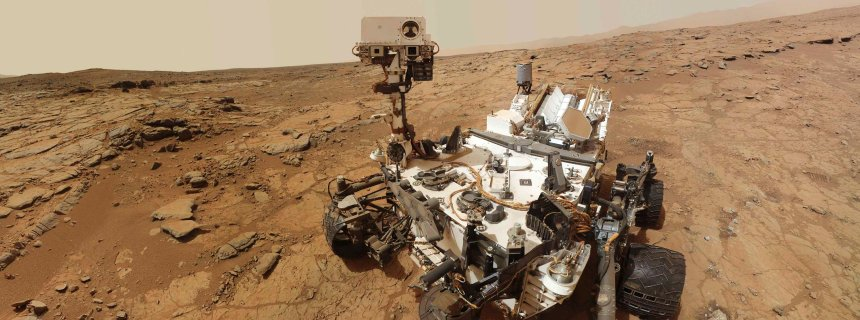
\includegraphics[width=\textwidth]{images/curiosity/curiosity}
\end{capfigure}

Für unseren EarthROVER waren folgende Funktionen geplant:
\begin{capitemize}[Funktionen EarthROVER (geplant)]
	\item Erkunden der Umgebung
	\item Erkennen und Merken von Hindernissen
	\item Den zurückgelegten Weg merken
	\item Wieder zum Ausgangspunkt zurückkehren
	\item Bilder von interessanten Objekten zu machen
	\item Einen Live-Stream von der Kamera liefern
	\item Einen Ball finden
	\item Den Ball aufheben mit Hilfe eines Greifarms
	\item Sensordaten, Bilder und Live-Stream über ein Web-Interface anbieten
	\item Den EarthROVER fernsteuern können
\end{capitemize}

\TODO{Sind das alle geplanten Funktionen?}

Von Vorne herein war klar, dass wir entweder aus zeitlichen oder aus technischen Gründen nicht alles umsetzen werden können.